\documentclass[reqno,a4paper,12pt]{amsart}

\usepackage{amsmath,amssymb,amsthm,geometry,xcolor,soul,graphicx}
\usepackage{titlesec}
\usepackage{enumerate}
\usepackage{lipsum}
\usepackage{listings}
\allowdisplaybreaks[4] %align公式跨页
\RequirePackage[most]{tcolorbox}
\usepackage{xeCJK}
\setCJKmainfont{Kai}

\geometry{left=0.7in, right=0.7in, top=1in, bottom=1in}



\renewcommand{\baselinestretch}{1.3}

\title{高等热力学与统计物理第六次作业}
\author{董建宇}

\begin{document}
\maketitle

\titleformat{\section}[hang]{\small}{\thesection}{0.8em}{}{}
\titleformat{\subsection}[hang]{\small}{\thesubsection}{0.8em}{}{}

\section{计算Maxwell分布下的最可几速度,平均速度和速度分布的宽度,即
\[
	\Delta v \equiv \sqrt{\langle (v - \langle v \rangle)^2 \rangle}
\]
将结果用绝对温度和分子质量表达。并算出氢气和氧气以上各量在室温下的数值。
}
\begin{tcolorbox}[breakable, colback = black!5!white, colframe = black]
Maxwell速度分布为:
\[
	f(\vec{v}) = \left( \frac{m}{2\pi kT} \right)^{3/2} 4\pi v^2 e^{-\frac{mv^2}{2kT}}.
\]
求导可得:
\[
	\frac{df}{dv} = \left( \frac{m}{2\pi kT} \right)^{3/2} 4\pi v e^{-\frac{mv^2}{2kT}}\left( 2 - \frac{mv^2}{kT} \right).
\]
令$\frac{df}{dv} = 0$,可以解得最可几速度为:
\[
	v_1 = \sqrt{\frac{2kT}{m}}.
\]
平均速度为:
\[
	\langle v \rangle = \int_0^{\infty} v f(\vec{v}) \,dv = \left( \frac{m}{2\pi kT} \right)^{3/2} 4\pi \int_0^\infty v^3 e^{-\frac{mv^2}{2kT}}\,dv = 4\pi \left( \frac{m}{2\pi kT} \right)^{3/2} 2\left( \frac{kT}{m} \right)^2 = \sqrt{\frac{8kT}{\pi m}}.
\]
速度平方的平均值为:
\[
	\langle v^2 \rangle = \int_0^\infty v^2 f(v)\,dv = \left( \frac{m}{2\pi kT} \right)^{3/2} 4\pi \int_0^\infty v^4e^{-\frac{mv^2}{2kT}}\,dv = \frac{3kT}{m}.
\]
则速度分布的宽度为:
\[
	\Delta v = \sqrt{\langle v^2 \rangle - \langle v \rangle^2} = \sqrt{\left(3 - \frac{8}{\pi}\right) \frac{kT}{m}}.
\]
在室温下$T = 300K$,氢气分子质量为:$m_{H_2} = 3.32 \times 10^{-24}g$,氧气分子质量为:$m_{O_2} = 5.32 \times 10^{-23}g$,代入数据可得,对于氢气有:
\[
	v_1 = 1.58 \times 10^3 m/s; ~~ \langle v \rangle = 1.782 \times 10^3 m/s; ~~ \Delta v = 752 m/s.
\]
对于氧气有:
\[
	v_1 = 395m/s; ~~ \langle v \rangle = 445m/s; ~~ \Delta v = 188m/s.
\]
\end{tcolorbox}

\section{由同一种分子组成的理想气体被隔膜分成两部分。每部分的体积,粒子数和温度如图所示。假设隔膜左右温度相同但密度不同,且系统与外界热绝缘。证明隔膜撤掉后气体的熵增加。\\
\begin{centering}
	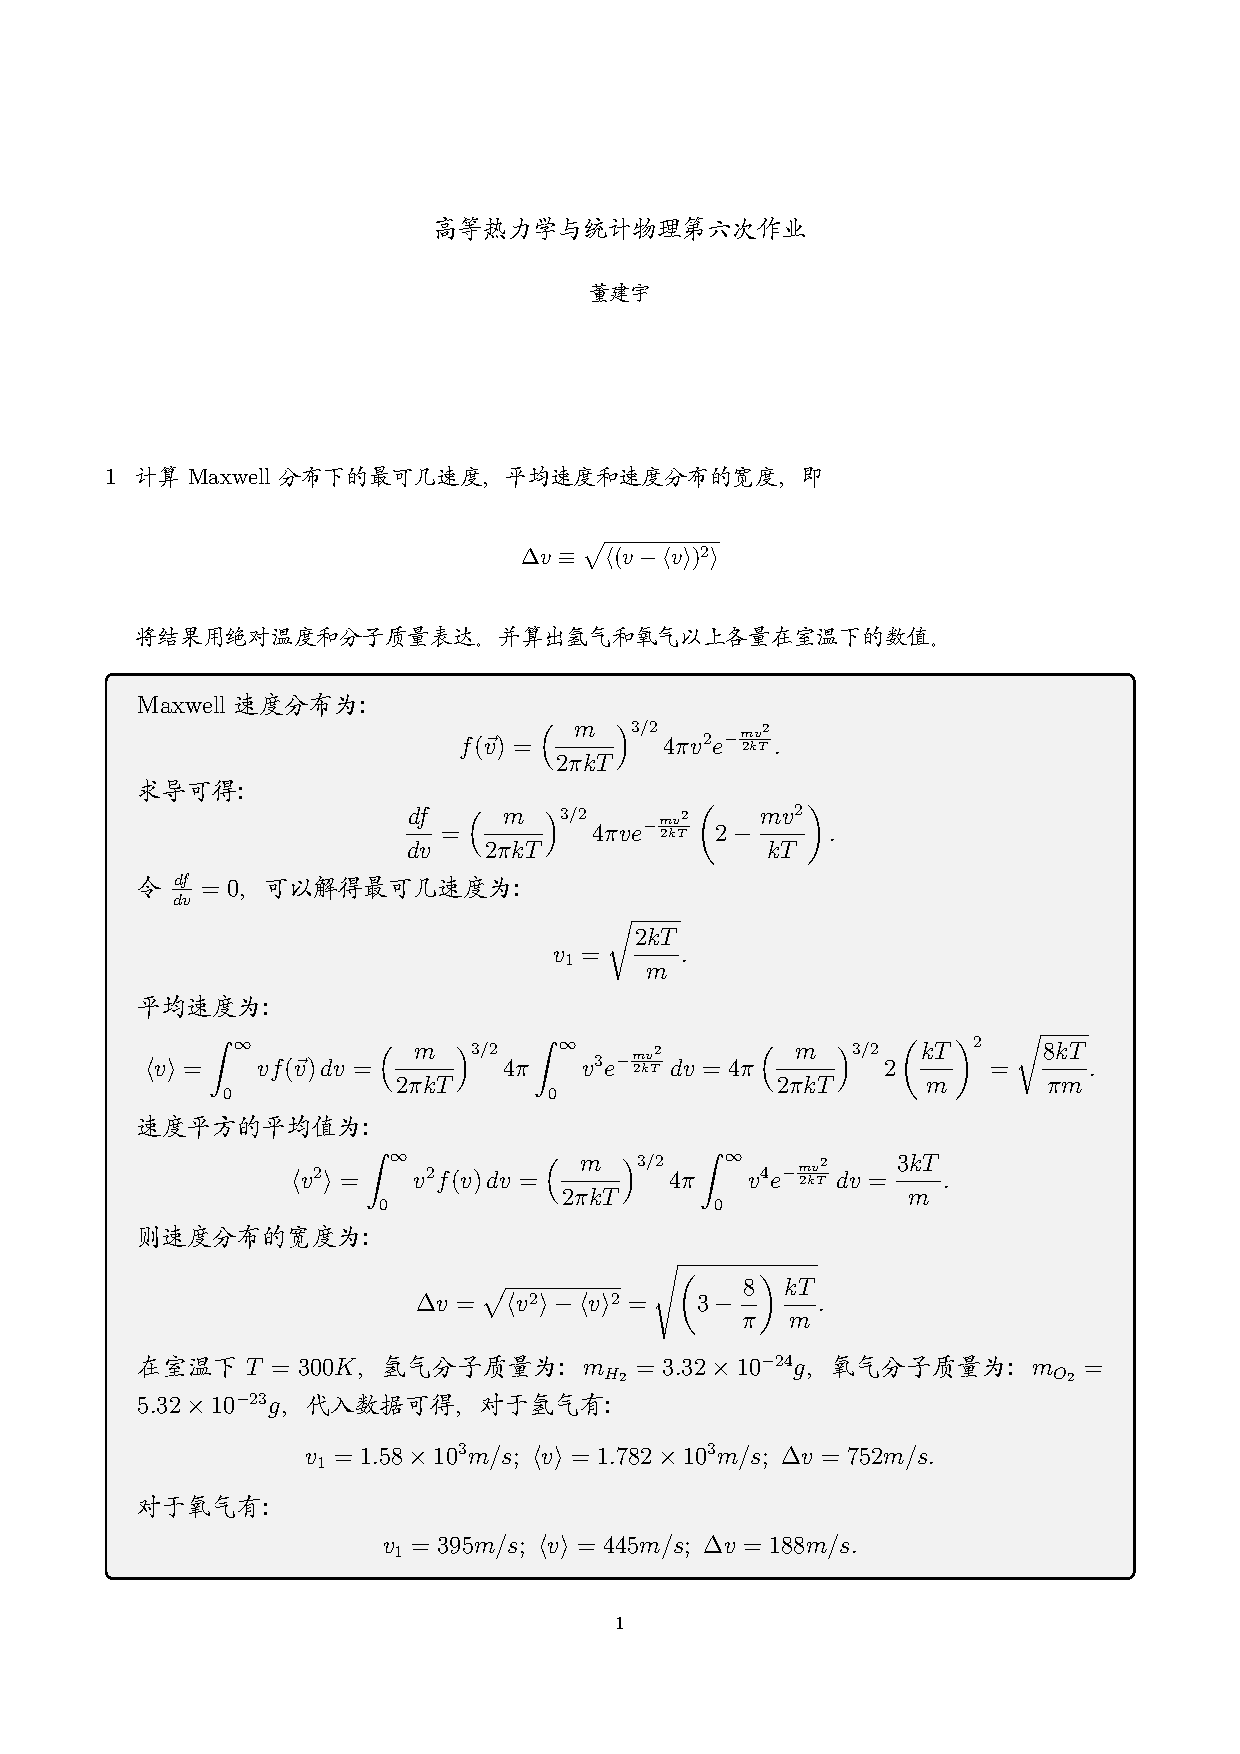
\includegraphics[scale = 0.13]{homework6.jpeg}
\end{centering}
}
\begin{tcolorbox}[breakable, colback = black!5!white, colframe = black]
由于气体为理想气体,则初态的熵为:
\[
	S_A = \frac{3}{2}N_Ak\ln \frac{2\pi mkT}{\hbar^2} + N_Ak\ln \frac{V_A}{N_A} + \frac{5}{2}N_Ak,
\]
\[
	S_B = \frac{3}{2}N_Bk\ln \frac{2\pi mkT}{\hbar^2} + N_Bk\ln \frac{V_B}{N_B} + \frac{5}{2}N_Bk.
\]
则初态系统的熵为:
\[
	S_0 = S_A + S_B = \frac{3}{2}(N_A+N_B)k\ln\frac{2\pi mkT}{\hbar^2} + \frac{5}{2}(N_A+N_B)k + N_Ak\ln \frac{V_A}{N_A} + N_Bk\ln \frac{V_B}{N_B}.
\]
隔膜撤掉后,气体分子总数为:$N = N_A + N_B$,温度为:$T$,体积为:$V = V_A+V_B$则气体的熵为:
\[
	S_1 = \frac{3}{2}(N_A+N_B)k\ln \frac{2\pi mkT}{\hbar^2} + \frac{5}{2}(N_A+N_B)k + (N_A+N_B)k\ln \frac{V_A+V_B}{N_A+N_B}.
\]
则熵变化量为:
\[
	\Delta S = S_1 - S_0 = (N_A+N_B)k\ln \frac{V_A+V_B}{N_A+N_B} - \left( N_Ak\ln \frac{V_A}{N_A} + N_Bk\ln \frac{V_B}{N_B} \right)
\]
令$x_1 = \frac{V_A}{N_A}$,$x_2 = \frac{V_B}{N_B}$,$\alpha = \frac{N_A}{N_A+N_B}$,$f(x) = \ln x$,则可以计算:
\[
	\frac{d^2f(x)}{dx^2} = -\frac{1}{x^2} < 0.
\]
即$f(x)$为凹函数(上凸)。则有对于任意的$\alpha \in (0,1)$,满足
\[
	f(\alpha x_1 + (1-\alpha) x_2) > \alpha f(x_1) + (1-\alpha)f(x_2).
\]
注意到熵的变化量为:
\[
	\Delta S = (N_A+N_B)k (f(\alpha x_1 + (1-\alpha) x_2) - \alpha f(x_1) + (1-\alpha)f(x_2)) > 0.
\]
则隔膜撤掉后气体的熵增加。
\end{tcolorbox}


\section{在高温条件下,即
\[
	\epsilon \equiv \frac{\hbar^2}{2IkT} << 1
\]
证明双原子气体的转动配分函数
\[
	q_r = \omega \left[ \frac{1}{\epsilon} + \frac{1}{3} + \frac{1}{15}\epsilon + \mathcal{O}(\epsilon^2) \right]
\]
和每个分子平均转动动能
\[
	u_r = kT\left[ 1 - \frac{1}{3}\epsilon - \frac{1}{45}\epsilon^2 + \mathcal{O}(\epsilon^3) \right]
\]
其中$\omega$为核自旋的简并度
\[
	\omega = \left\{
	\begin{aligned}
		&(2s_A+1)(2s_B+1), & AB \\
		&\frac{1}{2}(2s_A+1)^2, & AA
	\end{aligned}\right.
\]
提示:可用Euler-Maclaurin公式计算修正项
}
\begin{tcolorbox}[breakable, colback = black!5!white, colframe = black]
令$f(j) = (2j+1)e^{-\epsilon(j^2+j)}$,则有:
\[
	\int_0^{\infty} f(j)\,dj = \left. -\frac{1}{\epsilon}e^{-\epsilon(j^2+j)} \right\vert_0^\infty = \frac{1}{\epsilon}.
\]
\[
	f(0) = 1, ~~ f(\infty) = 0.
\]
\[
	\frac{df}{dj} = 2e^{-\epsilon(j^2+j)} - \epsilon(2j+1)^2e^{-\epsilon(j^2+j)}
\]
\[
	f^{(1)}(0) = 2-\epsilon, ~~ f^{(1)}(\infty) = 0.
\]
\[
	f^{(2)}(j) = \epsilon^2(2j+1)^3e^{-\epsilon(j^2+j)} - 6\epsilon(2j+1) e^{-\epsilon(j^2+j)}.
\]
\[
	f^{(3)}(j) = \left( -\epsilon^3(2j+1)^4 + 12\epsilon^2(2j+1)^2 - 12\epsilon \right)e^{-\epsilon(j^2+j)}.
\]
\[
	f^{(3)}(0) = (-\epsilon^3 + 12\epsilon^2 - 12\epsilon), ~~ f^{(3)}(\infty) = 0.
\]
则有:
\begin{align*}
	\sum_0^{\infty} f(j) =& \frac{1}{\epsilon} + \frac{1}{2} - \frac{1}{12}(2-\epsilon) + \frac{1}{720}(-\epsilon^3 + 12\epsilon^2 - 12\epsilon) \\ 
	=& \frac{1}{\epsilon} + \frac{1}{3} + \frac{1}{15}\epsilon + \mathcal{O}(\epsilon^2).
\end{align*}
对于AB型分子,$\Delta j = 1$,则有:
\begin{align*}
	q_r =& (2s_A+1)(2s_B+1)\sum_{j=0}^{\infty}(2j+1)e^{-\epsilon j(j+1)}\Delta j \\
	=& (2s_A+1)(2s_B+1) \left[ \frac{1}{\epsilon} + \frac{1}{3} + \frac{1}{15}\epsilon + \mathcal{O}(\epsilon^2) \right].
\end{align*}
对于AA型分子,$\Delta j = 2$,当$j$为偶数时则有:
\begin{align*}
	q_r =& (2s_A+1)^2 \sum_{j,\Delta j =2}(2j+1)e^{-\epsilon j(j+1)} \frac{\Delta j}{2} \\
	=& \frac{1}{2}(2s_A+1)^2 \sum_{i=0}^{\infty} (8i+2) e^{-\epsilon (4i^2+2i)}
\end{align*}
其中$i=j/2$。令$g(i) = (8i+2) e^{-\epsilon (4i^2+2i)}$,则可以计算:
\[
	\int_0^{\infty} g(i)\,di = \left. -\frac{1}{\epsilon}e^{-\epsilon(4i^2+2i)} \right\vert_0^\infty = \frac{1}{\epsilon}.
\]
\[
	g(0) = 2, ~~ g(\infty) = 0.
\]
\[
	g^{(1)} = (8-\epsilon(8i+2)^2) e^{-\epsilon(4i^2+2i)}.
\]
\[
	g^{(1)}(0) = 8-4\epsilon, ~~ g^{(1)}(\infty) = 0.
\]
\[
	g^{(3)} = \left( -\epsilon^3(8i+2)^4 + 24\epsilon^2(8i+2)^2 - 192 \epsilon \right) e^{-\epsilon(4i^2+2i)}
\]
\[
	g^{(3)}(0) = -\epsilon^3 + 24\epsilon^2 - 192\epsilon, ~~ g^{(3)}(\infty) = 0.
\]
则有:
\begin{align*}
	\sum_{i=1}^{\infty}g(i) =& \frac{1}{\epsilon} + 1 - \frac{1}{12}(8-4\epsilon) + \frac{1}{720}(-\epsilon^3 + 24\epsilon^2 - 192\epsilon) \\
	=& \frac{1}{\epsilon} + \frac{1}{3} + \frac{1}{15}\epsilon + \mathcal{O}(\epsilon^2).
\end{align*}
同理可知,当$j$为奇数时,令$k=(j-1)/2$,可以计算得相同结果。则有双原子气体的转动配分函数为:
\[
	q_r = \omega \left[ \frac{1}{\epsilon} + \frac{1}{3} + \frac{1}{15}\epsilon + \mathcal{O}(\epsilon^2) \right].
\]
其中核自旋简并度为:
\[
	\omega = \left\{
	\begin{aligned}
		&(2s_A+1)(2s_B+1), & AB \\
		&\frac{1}{2}(2s_A+1)^2, & AA
	\end{aligned}\right.
\]
则每个分子的平均转动动能为:
\[
	u_r = -\frac{\partial\ln q_r}{\partial\beta} = -\frac{\hbar^2}{2I}\frac{\partial \ln q_r}{\partial \epsilon} 
\]
可以计算:
\[
	\ln q_r = \ln \omega - \ln \epsilon + \ln\left( 1+\frac{\epsilon}{3} + \frac{\epsilon^2}{15} + \mathcal{O}(\epsilon^3) \right) = \ln \omega - \ln \epsilon + \frac{\epsilon}{3} + \frac{\epsilon^2}{90} + \mathcal{O}(\epsilon^3).
\]
则平均转动动能为:
\[
	u_r = \epsilon kT\left( \frac{1}{\epsilon} - \frac{1}{3} - \frac{1}{45}\epsilon + \mathcal{O}(\epsilon^2) \right) = kT\left( 1 - \frac{1}{3}\epsilon - \frac{1}{45}\epsilon^2 + \mathcal{O}(\epsilon^3) \right).
\]
\end{tcolorbox}


\end{document}